% !TEX TS-program = pdflatex
% !TEX encoding = UTF-8 Unicode
% !TEX spellcheck = en_US

\documentclass[11pt]{article}
\usepackage[utf8]{inputenc} 
\usepackage{geometry}
\geometry{a4paper}
% \usepackage[german]{babel}
\usepackage{mathtools}
\usepackage{amsfonts,amsmath,amssymb,amsthm, amsbsy}
\usepackage{tikz}
\usetikzlibrary{arrows}
\usetikzlibrary{fit}
\usepackage{subfigure}
\tikzstyle{vertex}=[circle,fill=black!25,minimum size=20pt,inner sep=0pt]
\tikzstyle{selected vertex} = [vertex, fill=red!24]
\tikzstyle{edge} = [draw,thick,->]
\tikzstyle{weight} = []
\usepackage{algorithmic}
\usepackage{listings}

\usepackage{graphicx}
\usepackage[parfill]{parskip}
\usepackage{booktabs} % for much better looking tables
\usepackage{array} % for better arrays (eg matrices) in maths
\usepackage{paralist} % very flexible & customisable lists (eg. enumerate/itemize, etc.)
\usepackage{verbatim} % adds environment for commenting out blocks of text & for better verbatim
\usepackage{subfig} % make it possible to include more than one captioned figure/table in a single float
\usepackage{amsfonts}
\usepackage{amsmath}
\usepackage{amsthm}
\usepackage{amssymb}
\usepackage{mathtools}
\usepackage{stmaryrd}
\usepackage{mathabx}
\usepackage[]{algorithm2e}
\usepackage{pdflscape}
\usepackage{dsfont}

\usepackage{proof}

\usepackage{pgf}
\usepackage{tikz}
\usetikzlibrary{matrix,positioning,automata,arrows,shapes,petri}
\tikzset{
place/.style={circle,thick,draw=black,minimum size=10mm},
transition/.style={rectangle,thick,draw=black,minimum width=3mm,inner ysep=5mm, fill=black}
}

\usepackage{xcolor}
\definecolor{secblue}{rgb}{0.18, 0.39, 0.77}
\definecolor{deepblue}{rgb}{0,0,0.5}
\definecolor{deepred}{rgb}{0.6,0,0}
\definecolor{deepgreen}{rgb}{0,0.5,0}

\usepackage{sectsty}
\allsectionsfont{\normalfont\sffamily\bfseries\color{secblue}}

%%% Aliases
\DeclarePairedDelimiter\floor{\lfloor}{\rfloor}
\DeclarePairedDelimiter\abs{\lvert}{\rvert}

% Command to declare a column vector. Param 1 is the dimension, then n elements follow
\newcount\colveccount
\newcommand*\colvec[1]{
        \global\colveccount#1
        \begin{pmatrix}
        \colvecnext
}
\def\colvecnext#1{
        #1
        \global\advance\colveccount-1
        \ifnum\colveccount>0
                \\
                \expandafter\colvecnext
        \else
                \end{pmatrix}
        \fi
}

\def\arraystretch{1.33}


\title{Computational Group Theory \\ Exercise Sheet 2}
\author{
	Franks, Billy Joe \\
	\texttt{b\_franks12@cs.uni-kl.de}
	\and 
	Bergsträßer, Pascal \\
	\texttt{p\_bergstra15@cs.uni-kl.de}
}

\newtheorem{theorem}{Satz}

\begin{document}
\maketitle
% !TeX root = root.tex
% !TeX spellcheck = en_US
\section{Classification of transitive actions}
\clearpage
% !TeX root = root.tex
% !TeX spellcheck = en_US
\section{Group theoretic complexity classes}

We are given two groups $G$ and $H$, by their generators. We then compute the Normalizer of $H$ in $G$, $N_G(H)$. Now $<H^{N_G(H)}>=H$ by definition of the normailzer. From this we can compute $H \cap N_G(H)$, by 3.11.2, which contains elements from $H \cap G$, and all elements from $H \cap G \subseteq N_G(H)$ obviously, this shows the claim.

\clearpage
% !TeX root = root.tex
% !TeX spellcheck = en_US
\section{Centralizers}
\subsection*{a)}
Let $G \leq \text{Sym}(\Omega)$ be semiregular. We show that $C_{\text{Sym}(\Omega)}(G)$ is transitive.

First we show that $C_{\text{Sym}(\Omega)}(G)$ acts transitively on every orbit. Let $\alpha \in \Omega$ be arbitrary and $\beta \in \alpha^G$ be an element in the orbit of $\alpha$. We define $c \in \text{Sym}(\Omega)$ s.t. $\alpha^c = \beta$ as follows:
\[ \gamma^c := 
	\begin{cases} 
      \beta^g &, \gamma = \alpha^g \text{ for some } g \in G \\
      \gamma &, \gamma \in \Omega \setminus \alpha^G \\
   \end{cases} \]
To show that $c$ is well-defined, let $g, g^\prime \in G$ s.t. $\alpha^g = \gamma = \alpha^{g^\prime}$. Then, $g (g^\prime)^{-1} \in G_\alpha$ which implies that $g (g^\prime)^{-1} = e$ since $G$ is semiregular. Hence, $g = g^\prime$ and therefore $\beta^g = \beta^{g^\prime}$.

The function $c$ is bijective, since if $\beta^g = \beta^{g^\prime}$ then $g (g^\prime)^{-1} \in G_\beta$. So, $g = g^\prime$ and $\beta^g = \beta^{g^\prime}$. Thus, $c$ maps injectively from $\Omega$ to $\Omega$ which means that $c$ is bijective.

Next, we show that $c \in C_{\text{Sym}(\Omega)}(G)$. Let $h \in G$ and $\gamma \in \Omega$ be arbitrary. If $\gamma \in \alpha^G$ then there exists $g \in G$ s.t. $\alpha^g = \gamma$. It follows that
\[ \gamma^{hc} = \alpha^{ghc} = \beta^{gh} = \gamma^{ch}. \]
If $\gamma \in \Omega \setminus \alpha^G$, then
\[ \gamma^{hc} = \gamma^h = \gamma^{ch} \]
since $\gamma^h \in \Omega \setminus \alpha^G$.

Moreover, it holds that $\alpha^c = (\alpha^e)^c = \beta^e = \beta$.

By Lemma 3.12.10, the orbits of $G$ are pairwise equivalent since $\text{fix}(G_\alpha) = \Omega$ for all $\alpha \in \Omega$. Thus, by Lemma 3.12.8 for every two orbits there exists $c \in C_{\text{Sym}(\Omega)}(G)$ that maps one orbit to the other. So, for arbitrary $\alpha, \beta \in \Omega$ we use $c_1 \in C_{\text{Sym}(\Omega)}(G)$ that maps $\alpha^G$ to $\beta^G$ and $c_2 \in C_{\text{Sym}(\Omega)}(G)$ to map $\alpha^{c_1}$ to $\beta$ in the same orbit. Hence, $\alpha^{c_1 c_2} = \beta$ with $c_1 c_2 \in C_{\text{Sym}(\Omega)}(G)$. This means that $C_{\text{Sym}(\Omega)}(G)$ is transitive.

\subsection*{b)}
Let $H,G \leq \text{Sym}(\Omega)$ s.t. $G$ normalizes $H$. To show that $G$ normalizes $C_{\text{Sym}(\Omega)}(H)$, let $c \in C_{\text{Sym}(\Omega)}(H)$, $g \in G$ and $h \in H$ be arbitrary. Then,
\[ (g^{-1}cg)^{-1}h(g^{-1}cg) = g^{-1}c^{-1}(ghg^{-1})cg = g^{-1}ghg^{-1}g = h \]
since $ghg^{-1} \in H$ as $G$ normalizes $H$. This means that $g^{-1}cg \in C_{\text{Sym}(\Omega)}(H)$. Thus, $G$ normalizes $C_{\text{Sym}(\Omega)}(H)$.

\subsection*{c)}

\clearpage
% !TeX root = root.tex
% !TeX spellcheck = en_US
\section{Magic Solid}
\clearpage
% !TeX root = root.tex
% !TeX spellcheck = en_US
\section{GAP-exercise}
\subsection*{a)}
To compute the number of primitive permutation groups up to permutational equivalence, we use the GAP function \textit{NrPrimitiveGroups}. 

\lstinputlisting[language=gap]{ex5a.g}

Then for degrees $d = \{1,\dots, 100\}$ we get

\hspace*{-1cm}
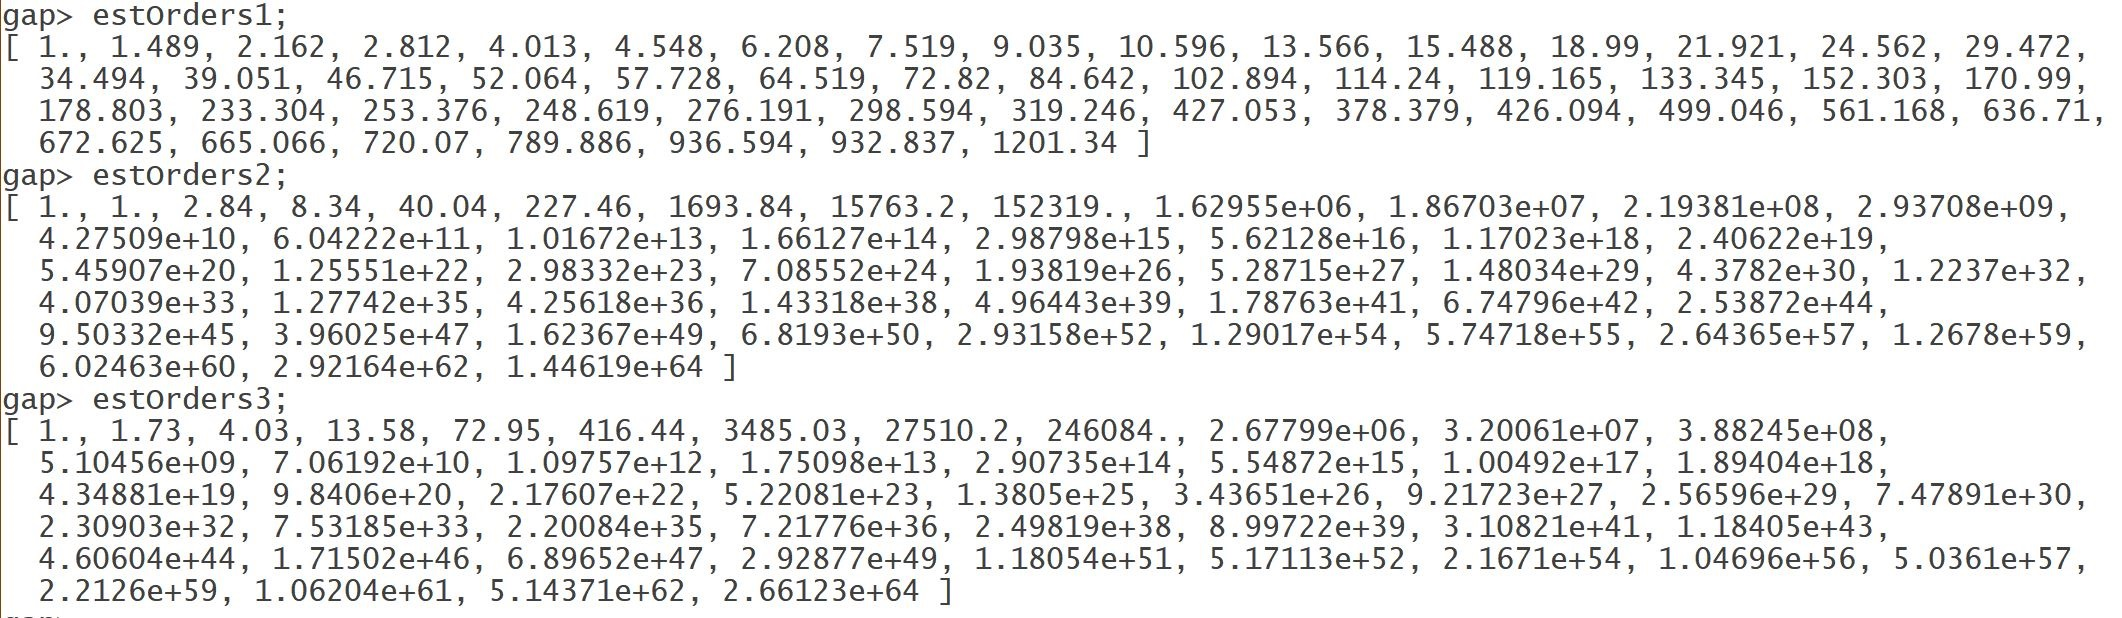
\includegraphics[width=17cm]{ex5}

\subsection*{b)}
We determine the possible number of minimal normal subgroups of primitive permutation groups of degree $d = \{1,\dots, 50\}$ as follows:

\lstinputlisting[language=gap]{ex5b.g}

We obtain that all groups except the trivial group have exactly one minimal normal subgroup.

\subsection*{c)}
Based on the results from b) we state the conjecture that primitive permutation groups except the trivial group have a unique minimal normal subgroup.
\end{document}
